%============================================================
\section{Nombre: LLuvia de lava.} \label{hab.LLuviaLava}
\subsection{Descripción}
Caen bolas de lava del cielo en posiciones aleatorias. Las bolas de lava se destruyen al colisionar con el suelo, con una plataforma o con el jugador. Cuando una de las bolas de lava colisiona con el jugador disminuye la cantidad de vida del jugador, es decir cada bola de lava genera daño de manera individual. Las bolas de lava no pueden destruir las plataformas o el suelo al colisionar contra estas.
\subsection{Portador}
Itztlacoliuhqui (ver apartado \ref{per:itztlacoliuhqui}), Mictlantechtli (ver apartado \ref{per:mictlantechtli}).	
\subsection{Esquema}	
			Ver figura \ref{fig:lluviaL}.
			\begin{figure}
				\centering
				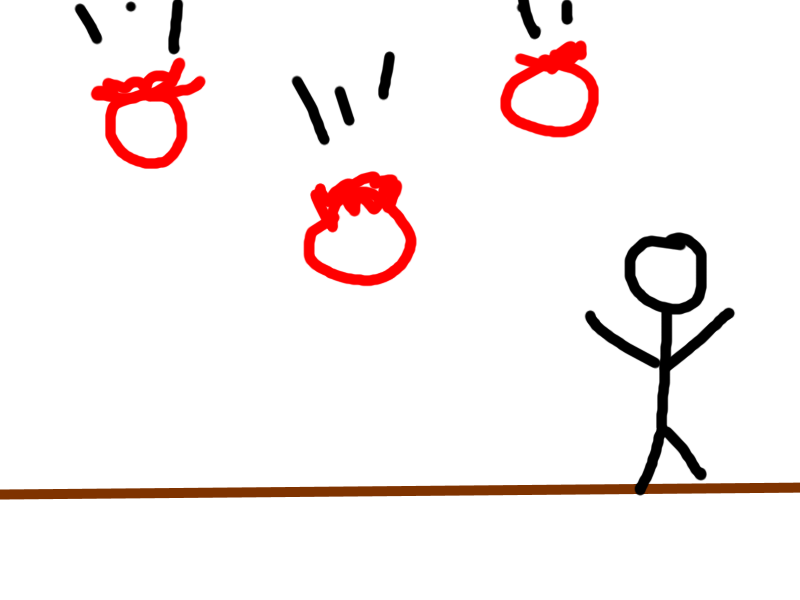
\includegraphics[height=0.2 \textheight]{Imagenes/lluviaL}
				\caption{Lluvia de lava.}
				\label{fig:lluviaL}
			\end{figure}